% Energy levels of a fluor molecule
% Author: David Fokkema
\documentclass{article}
\usepackage{tikz}
%%%<
\usepackage{verbatim}
%\usepackage[active,tightpage]{preview}
%\PreviewEnvironment{center}
%\setlength\PreviewBorder{10pt}%
%%%>
\begin{comment}
:Title: Energy levels of a fluor molecule
:Tags: Physics;Styles;Diagrams;Foreach;Clipping;Intersections
:Author: David Fokkema
:Slug: fluor-energy-levels

In particle physics, the most important experimental problem is that of
detecting particles.  A cheap and highly efficient solution is using
*scintillators*.  These kinds of detectors emit light when a charged
particle traverses the detector.  The light-emitting process is depicted
in this figure.  The layout was inspired by [this wikipedia
graphic](http://en.wikipedia.org/wiki/File:Pistates.svg).  The TikZ code
in my version is a bit complex, mainly due to manual layout tweaks,
shifting some positions here and there.  The figure shown here is a minor
revision of the one included in
[my PhD thesis](http://dx.doi.org/10.3990/1.9789036534383).
\end{comment}

\usetikzlibrary{calc,arrows,decorations.pathmorphing,intersections}
\usepackage[font={small,sf},labelfont={bf},labelsep=endash]{caption}
\usepackage{sansmath}
\begin{document}
\begin{center}
  \sansmath
  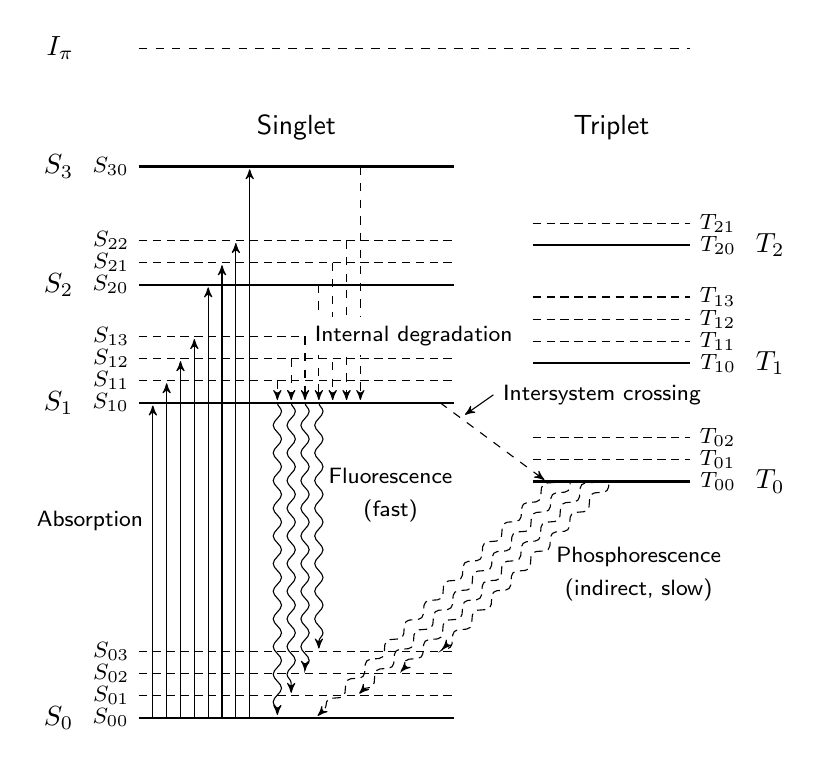
\begin{tikzpicture}[
    font=\sffamily,
    level/.style={black,thick},
    sublevel/.style={black,densely dashed},
    ionization/.style={black,dashed},
    transition/.style={black,->,>=stealth',shorten >=1pt},
    radiative/.style={transition,decorate,decoration={snake,amplitude=1.5}},
    indirectradiative/.style={radiative,densely dashed},
    nonradiative/.style={transition,dashed},
  ]
  \coordinate (sublevel) at (0, 8pt);

  % Singlet levels
  \coordinate (S00) at (0, -1);
  \coordinate (S01) at ($(S00) + (sublevel)$);
  \coordinate (S02) at ($(S00) + 2*(sublevel)$);
  \coordinate (S03) at ($(S00) + 3*(sublevel)$);
  \coordinate (S10) at (0, 3);
  \coordinate (S11) at ($(S10) + (sublevel)$);
  \coordinate (S12) at ($(S10) + 2*(sublevel)$);
  \coordinate (S13) at ($(S10) + 3*(sublevel)$);
  \coordinate (S20) at (0, 4.5);
  \coordinate (S21) at ($(S20) + (sublevel)$);
  \coordinate (S22) at ($(S20) + 2*(sublevel)$);
  \coordinate (S30) at (0, 6);

  % Draw main levels
  \foreach \level/\text in {00/0, 10/1, 20/2, 30/3}
    \draw[level] (S\level) node[left=20pt] {$S_\text$} node[left]
      {\footnotesize $S_{\level}$} -- +(4, 0);

  % Draw sublevels
  \foreach \sublevel in {01,02,03,11,12,13,21,22}
    \draw[sublevel] (S\sublevel) node[left]
      {\footnotesize $S_{\sublevel}$} -- +(4, 0);

  \node at (2, 6.5) {Singlet};

  % Triplet levels
  \coordinate (T00) at (5, 2);
  \coordinate (T01) at ($(T00) + (sublevel)$);
  \coordinate (T02) at ($(T00) + 2*(sublevel)$);
  \coordinate (T03) at ($(T00) + 3*(sublevel)$);
  \coordinate (T10) at (5, 3.5);
  \coordinate (T11) at ($(T10) + (sublevel)$);
  \coordinate (T12) at ($(T10) + 2*(sublevel)$);
  \coordinate (T13) at ($(T10) + 3*(sublevel)$);
  \coordinate (T20) at (5, 5);
  \coordinate (T21) at ($(T20) + (sublevel)$);

  % Draw main levels
  \foreach \level/\text in {00/0, 10/1, 20/2}
    \draw[level] (T\level) -- +(2, 0)
      node[right=20pt] {$T_\text$}
      node[right] {\footnotesize $T_{\level}$};

  % Draw sublevels
  \foreach \sublevel in {01,02,11,12,13,21}
    \draw[sublevel] (T\sublevel) -- +(2, 0) node[right]
      {\footnotesize $T_{\sublevel}$};

  \node at (6, 6.5) {Triplet};

  % Ionization level
  \draw[ionization] (0, 7.5) node[left=20pt] {$I_\pi$} -- +(7, 0);

  % Excitations
  \foreach \i/\from/\to in {1/S00/S10, 2/S00/S11, 3/S00/S12, 4/S00/S13,
                            5/S00/S20, 6/S00/S21, 7/S00/S22, 8/S00/S30}
    \draw[transition] ([xshift=\i*5pt] \from) -- ([xshift=\i*5pt] \to);

  % Radiative decay (fluorescence)
  \foreach \i/\from/\to in {1/S10/S00, 2/S10/S01, 3/S10/S02, 4/S10/S03}
    \draw[radiative] ([xshift=(\i+9)*5pt] \from) --
      ([xshift=(\i+9)*5pt] \to);

  % Nonradiative decay (internal degradation)
  \foreach \i/\from/\to in {1/S11/S10, 2/S12/S10, 3/S13/S10, 4/S20/S10,
                            5/S21/S10, 6/S22/S10, 7/S30/S10}
    \draw[nonradiative] ([xshift=(\i+9)*5pt] \from) --
      ([xshift=(\i+9)*5pt] \to);

  % Radiative decay (phosphorescence)
  %
  % There is some magic going on to prevent an irritating optical effect.
  % If the (start) coordinate is taken to be simply (Tstart), the wiggly
  % lines start at the T00 level.  Because of their differing lengths
  % however, the wiggles start to form a distracting pattern.  Therefore,
  % the lines are extended a bit (-\i*5pt) to show a pleasing effect.  They
  % are clipped so the transition still starts at T00.  If you want to
  % observe the optical effect, include this line at the correct location:
  %   \coordinate (start) at (Tstart);
  \begin{scope}
    \clip (S00) -- +(7, 0) |- (T00) -| (S00);
    \foreach \i/\level in {1/(S00), 2/(S01), 3/(S02), 4/(S03)} {
      \coordinate (Tstart) at ([xshift=\i*7pt] T00);
      \coordinate (end) at ($(Tstart) + (-135:4.5)$);
      \coordinate (start) at ($(Tstart)!-\i*5pt!(end)$);
      \path[name path=trans] (start) -- (end);
      \path[name path=ground] \level -- +(5, 0);
      \draw[indirectradiative,name intersections={of=trans and ground}]
        (start) -- (intersection-1);
    }
  \end{scope}

  % Labels (curious coordinates are due to manual placement adjustments)
  \node[left] at (5pt, 1.5) {\footnotesize Absorption};
  \node[right,align=center] at (13*5pt, 2cm - 5pt)
    {\footnotesize Fluorescence\\\footnotesize (fast)};
  \node[right,align=center] at (5cm + 5pt, 1cm - 5pt)
    {\footnotesize Phosphorescence\\\footnotesize (indirect, slow)};
  \node[right,fill=white,align=left] at ([xshift=12*5pt] S13)
    {\footnotesize Internal degradation};

  % Intersystem crossing
  \draw[nonradiative,name path=crossing] ($(S10) + (4, 0) - (5pt, 0)$) --
    ([xshift=5pt] T00);
  \coordinate (crosslabel) at (4.5, 3.1);
  \node[right,fill=white] at (crosslabel) {\footnotesize Intersystem crossing};
  \path[name path=arrow] (crosslabel) -- +(-145:1cm);
  \draw[->,>=stealth',shorten >=2pt,
    name intersections={of=crossing and arrow}]
    (crosslabel) -- (intersection-1);
  \end{tikzpicture}
  \captionof{figure}{Typical energy levels for $\pi$-orbitals of a fluor
    molecule. Spin singlet~($S$) and triplet~($T$) states are separated for
    clarity. The ionization level $I_\pi$ is shown at the top.  Excited states
    as well as vibrational sublevels (dashed horizontal lines) are shown. 
    Internal degradation is a non-radiative process, while fluorescence and
    phosphorescence are radiative decays.  The decay $T_0 \to S_0$, however,
    is indirect, by interactions with other molecules.}
\end{center}
\end{document}
